\section{Our Contributions}

We will present the SHE problem as an optimal control one, where the optimization variable is the signal $u(\tau)$ defined in the entire interval $[0,\pi)$. 
%
In particular, we will describe how the Fourier coefficients of the function $u(\tau)$ can be seen as the final state of a system controlled by $u (\tau)$. Hence, the optimization is performed among all the possible functions that satisfy $|u(\tau)|<1 $ and can control the final state at the desired Fourier coefficients. Then we will show how to design a control problem so that the solution is a step function.
 
In this way, we can reformulate Problem \ref{pb:SHEp} as follows.
\newline
In this formulation, the SHE problem converts in a minimization problem with restrictions which can be solved by well-known techniques. Since the problem has several minimizers, we shall solve it employing global optimizers. Furthermore, since the choice of the waveform is arbitrary, we shall proceed in the same way for each possible waveform. 

\subsection{Reformulation of SHE problem as optimal control problem}

%As we anticipated in Section \ref{Section1}, the main contribution of the present paper is to provide a novel and alternative approach to the SHE problem, based on optimal control. As we shall see, this methodology will allow us avoiding the choice of the waveform, as the optimization process selects the most convenient one in each case. 
%\newline

Teniendo en cuenta tenemos todos los elementos considerados en la definición del Problema \ref{pb:SHEp}, introducimos el siguiente sistema dinámico:

\begin{equation}\label{eq:CauchyReversed}
    \begin{cases}
        \displaystyle\dot{\bm{x}}(\tau) = -\frac 2\pi\bm{\mathcal{D}}(\tau)u(\tau),  & \tau \in [0,\pi)
        \\[6pt]
        \bm{x}(0) = \bm{x}_0
    \end{cases},
\end{equation}
Where $\bm{x}(t) \in \mathbb{R}^{N_a + N_b}$ and $\bm{\mathcal{D}}(\tau) \in  \mathbb{R}^{N_a + N_b}$ are:
\begin{align*}
	\bm{x}(\tau) = \begin{bmatrix} \bm{\alpha}(\tau) \\ \bm{\beta}(\tau) \end{bmatrix}, \quad
	\bm{\mathcal{D}}(\tau) = \begin{bmatrix} \bm{\mathcal{D}}^\alpha(\tau) \\ \bm{\mathcal{D}}^\beta(\tau) \end{bmatrix}     
\end{align*}
y donde:
\begin{align*}
	\bm{\mathcal{D}}^\alpha(\tau) = 
	\begin{bmatrix} 
		\cos(e_a^1\tau) \\ \cos(e_a^2\tau) \\ \vdots \\ \cos(e_a^{N_a}\tau) 
	\end{bmatrix},
	\quad \bm{\mathcal{D}}^\beta(\tau) = 
	\begin{bmatrix} 
		\sin(e_b^1\tau) \\ \sin(e_b^2\tau) \\ \vdots \\ \sin(e_b^{N_b}\tau) 
	\end{bmatrix} 
\end{align*}
with $\bm{\mathcal{D}}^\beta(\tau) \in \mathbb{R}^{N_a} $ and $ \bm{\mathcal{D}}^\beta(\tau) \in \mathbb{R}^{N_b}$, and where the set $\mathcal{E}_a$ and $\mathcal{E}_b$ are:
\begin{align*}
	\mathcal{E}_a = \{e_a^1,e_a^2,e_a^3,\dots,e_a^{N_a}\}, \quad \mathcal{E}_b = \{e_b^1,e_b^2,e_b^3,\dots,e_b^{N_b}\}    
\end{align*}
%
Además proponemos el siguiente problem de control:
\vspace{1em}
\begin{problem}\label{pb:SHEpControl}
    Let $\mathcal{U}$ be defined as in \eqref{eq:Udef} and let $\mathcal{E} _a $ and $\mathcal{E} _b $ be two sets of odd numbers with cardinalities $|\mathcal{E}_a| = N_a $ and $ |\mathcal{E} _b| = N_b$, respectively. Given the vectors $\bm{a}_T \in \mathbb{R}^{N_a}$ and $\bm{b}_T \in \mathbb{R}^{N_b} $, let us define $\bm{x}_0=[\bm{a}_T,\bm{b}_T]^\top \in \mathbb{R}^{N_a}\times\mathbb{R}^{N_b}$. We look for $u:\in [0,\pi)\to\mathcal{U}$ such that the solution of \eqref{eq:CauchyReversed} with initial datum $\bm{x}(0)=\bm{x}_0$ satisfies $\bm{x}(\pi)=0$.
\end{problem}
\vspace{1em}

\begin{theorem}
    El control óptimo $u(\tau)$, solución del Problema \ref{pb:SHEpControl}, es el función constante a trozos que resuleve el Problema \ref{pb:SHEp}.   
\end{theorem}

\begin{figure}[ht!] 
    \centering
    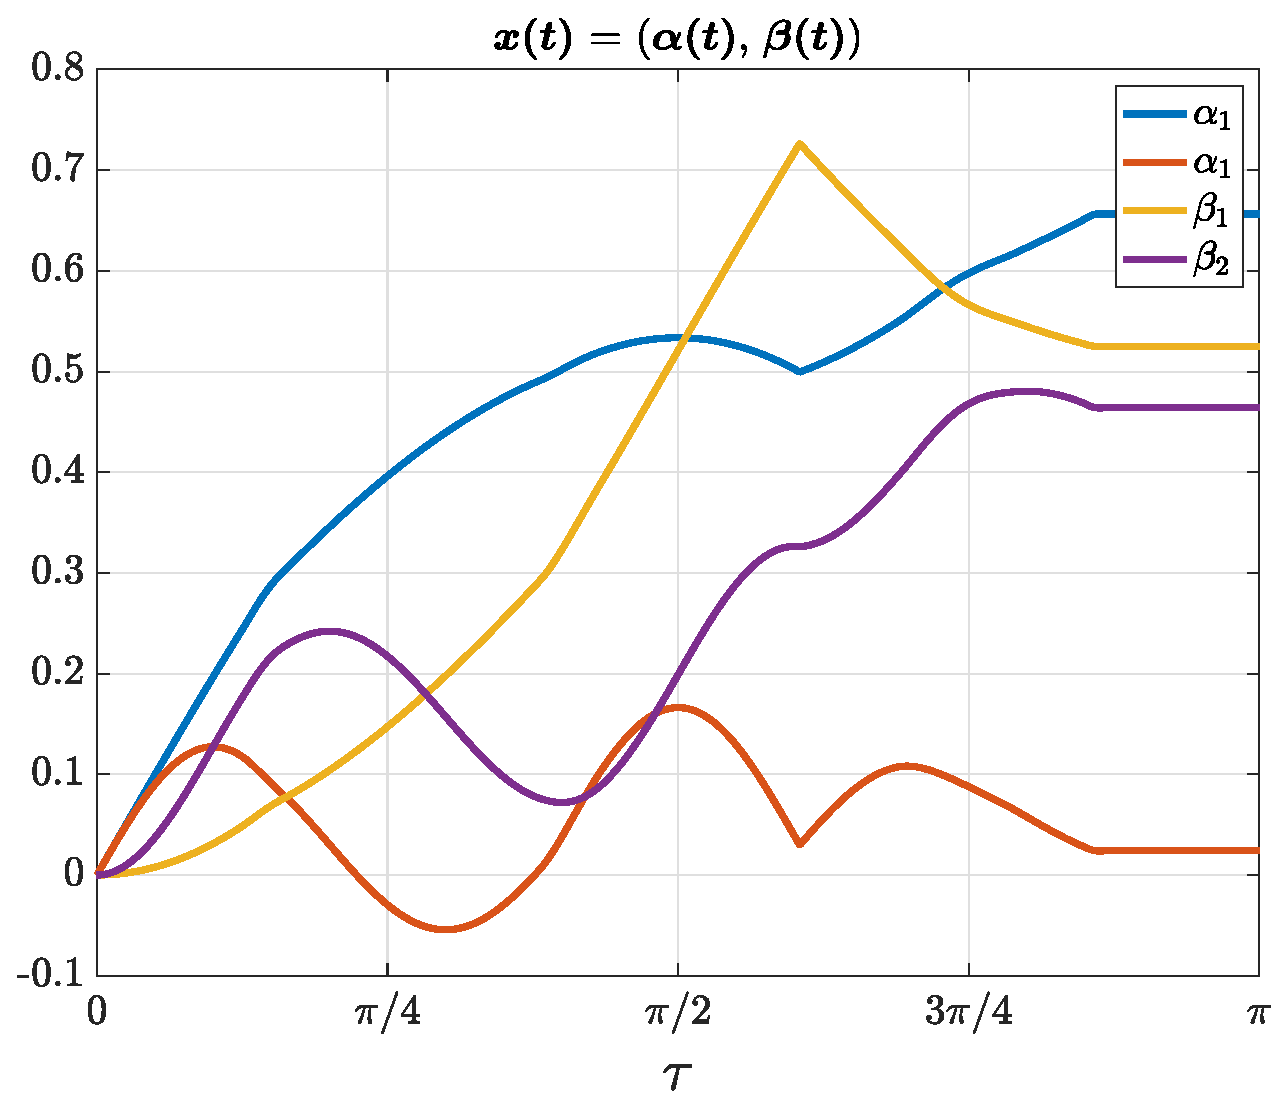
\includegraphics[scale=0.35]{img/fig02.eps}
    \caption{Evolución del sistema dinámico con los conjuntos $\mathcal{E}_a = \{1,2\}$ y $\mathcal{E}_b = \{1,2\}$ considerando el control $u(\tau)$ presentado en la Figura \ref{fig:exampleSHE}. Además mostramos las posiciones de los ángulos de conmutación $\bm{\phi}$.}
\end{figure}

\vspace{1em}
\begin{remark}[Quarter-wave symmetry]
    We shall mention that, in the SHE literature, it is usual to distinguish among the half-wave symmetry problem (addressed in the present paper) and the quarter-wave symmetry one in which
    \begin{align*}
        u\left(\tau + \frac \pi2\right) = -u(\tau)\quad \mbox{for all}\; \tau \in \left[0,\frac \pi2\right).
    \end{align*}
    In quarter-wave symmetry, the SHE problem simplifies, as the Fourier coefficients $\{a_i\}_{i\in\mathcal E_a}$ turn out to be all zero. Hence, only the phases of the converter's signal can be controlled, while the half-wave SHE allows to deal with the amplitudes as well. It is worth to remark nonetheless that our optimal control formulation can be easily adapted to the quarter-wave symmetry problem by simply replacing the Fourier coefficients \eqref{eq:an} with
    \begin{align*}
        a_i = 0, \quad\quad b_j = \frac{4}{\pi} \int_0^{\frac \pi4} u(\tau)  \sin(j \tau)\,d\tau.
    \end{align*}
    Entonces podemos introducir el siguiente sistema dinámico:
    \begin{gather}
        \begin{cases}
            \displaystyle \dot{\bm{\beta}}(\tau) = \frac 2\pi \bm{\mathcal{D}}^\beta(\tau) u(\tau), & \tau \in [0,\pi/2)
            \\[6pt]
            \bm{\beta}(0) = \bm{b}_T
        \end{cases}\label{eq:CauchyReversed_4sym}
    \end{gather}
    Además del siguiente problema de control:
    \vspace{0.5em}
    \begin{problem}\label{pb:SHEpControl_4sym}
        Let $\mathcal{U}$ be defined as in \eqref{eq:Udef} and let $\mathcal{E} _b $ be a set of odd numbers with cardinality $ |\mathcal{E} _b| = N_b$. Given the vector $\bm{b}_T \in \mathbb{R}^{N_b} $. We look for $u:\in [0,\pi/2)\to\mathcal{U}$ such that the solution of \eqref{eq:CauchyReversed_4sym} with initial datum $\bm{x}(0)=\bm{x}_0$ satisfies $\bm{x}(\pi)=0$.
    \end{problem}
    Donde de la misma forma que en el problema con simetría de media onda la solución de este problema es también solución del problema SHE con simetría de cuarto de onda.
\end{remark}


%As we anticipated in Section \ref{Section3}, the SHE problem is equivalent to controlling a dynamical system associated with the Fourier coefficients \eqref{eq:an}. In this section, we present a rigorous formulation of this mentioned control problem and we analyze some relevant properties. 

In what follows, for a given vector $\bm{v}\in\mathbb{R}^d$, we shall always denote by $\|\bm{v}\|$ the euclidean norm $\|\bm{v}\|_{\mathbb{R}^d}$.
\newline


\begin{problem}[OCP for SHE]\label{pb:OCP1}
Let $\mathcal U$ be defined as in \eqref{eq:Udef}. Given two sets of odd numbers $\mathcal {E}_a $ and $\mathcal {E}_b $ with cardinality $N_a$ and $N_b$, respectively, and given the target $\bm{x}_T\in \mathbb{R}^{N_a+N_b}$, we look for the function $u(\tau):[0,\pi)\to \mathcal U$ solution of the optimal control problem  
\begin{align*}
	&\min_{u \in \mathcal{U}}\;\frac 12 \|\bm{x}(\pi)\|^2
	\\
    &\notag \text{subject to: }\quad \begin{cases}
            \displaystyle \dot{\bm{x}}(\tau) = -\frac 2\pi\bm{\mathcal{D}}(\tau) u(\tau),  & \tau \in [0,\pi)\\[6pt]
            \bm{x}(0) = \bm{x}_0
    \end{cases}
    \end{align*}
\end{problem}
The solution of Problem \ref{pb:OCP1} may be quite complex to be obtained, due to the restriction on the admissible control values. 

In order to bypass this difficulty, following a standard optimal control approach, we can formulate an equivalent minimization problem in which, instead of looking for $u\in\mathcal U$, we simply require that $|u|<1$ and we introduce a penalization term to ensure that $u$ is a piece-wise constant function (\textcolor{red}{digital control}). 

\vspace{0.5em}
\begin{definition}[Digital control of set $\mathcal{U}$]
A control $u(\tau)$ is called digital if, for each time $\tau\geq 0$, it only takes values in the finite set of real number $\mathcal{U}$ except a finite set of values.  
\end{definition}
%
This alternative optimal control problem, which can be solved more easily by employing standard tools, reads as follows:
\newline
\begin{problem}[Penalized OCP for SHE]\label{pb:OCP2}
Fix $\epsilon>0$. Given two sets of odd numbers $\mathcal E_a $ and $\mathcal E_b $ and the target $\bm{x}_T \in \mathbb {R}^{N_a + N_b}$, we look for the  function $u:[0,\pi)\to\mathcal U$ as the solution of:
\begin{align*}
	&\min_{|u|<1} \Bigg[\frac 12 \|\bm{x}(\pi) \|^2+ \epsilon \int_0^{\pi} \mathcal{L}(u(\tau)) d\tau \Bigg]  
\end{align*}
under the dynamics given by \eqref{eq:CauchyReversed}.
\end{problem}

In Problem \ref{pb:OCP2}, the penalization function $\mathcal L: \mathbb{R} \rightarrow \mathbb{R}$ will be chosen such that the optimal control $u^*$ only takes values in $\mathcal U$. Furthermore, the parameter $\epsilon$ should be small so that the solution minimizes the distance from the final state and the target.

%Next we will study the optimality conditions of the problem, for a general $\mathcal L$, and then specify how $\mathcal L$ should be so that the optimal control $u^*$ only takes the allowed values in $\mathcal U$.


\subsection{SHE bi-nivel via OCP (Bang-Bang Control)} 

\begin{theorem}\label{th:bang-bang}
    Dado el Problema \ref{pb:OCP2} con el conjunto admisible de control $ \ \mathcal{U} = \{-1,1\}$. Si la función $\mathcal{L}$ es concava en el intervalo $[-1,1]$ del Problema \ref{pb:OCP2}, entonces la solución de problema es un control digital del conjunto $\mathcal{U} =  \{-1,1\}$.
\end{theorem}

\begin{figure} 
    \centering
    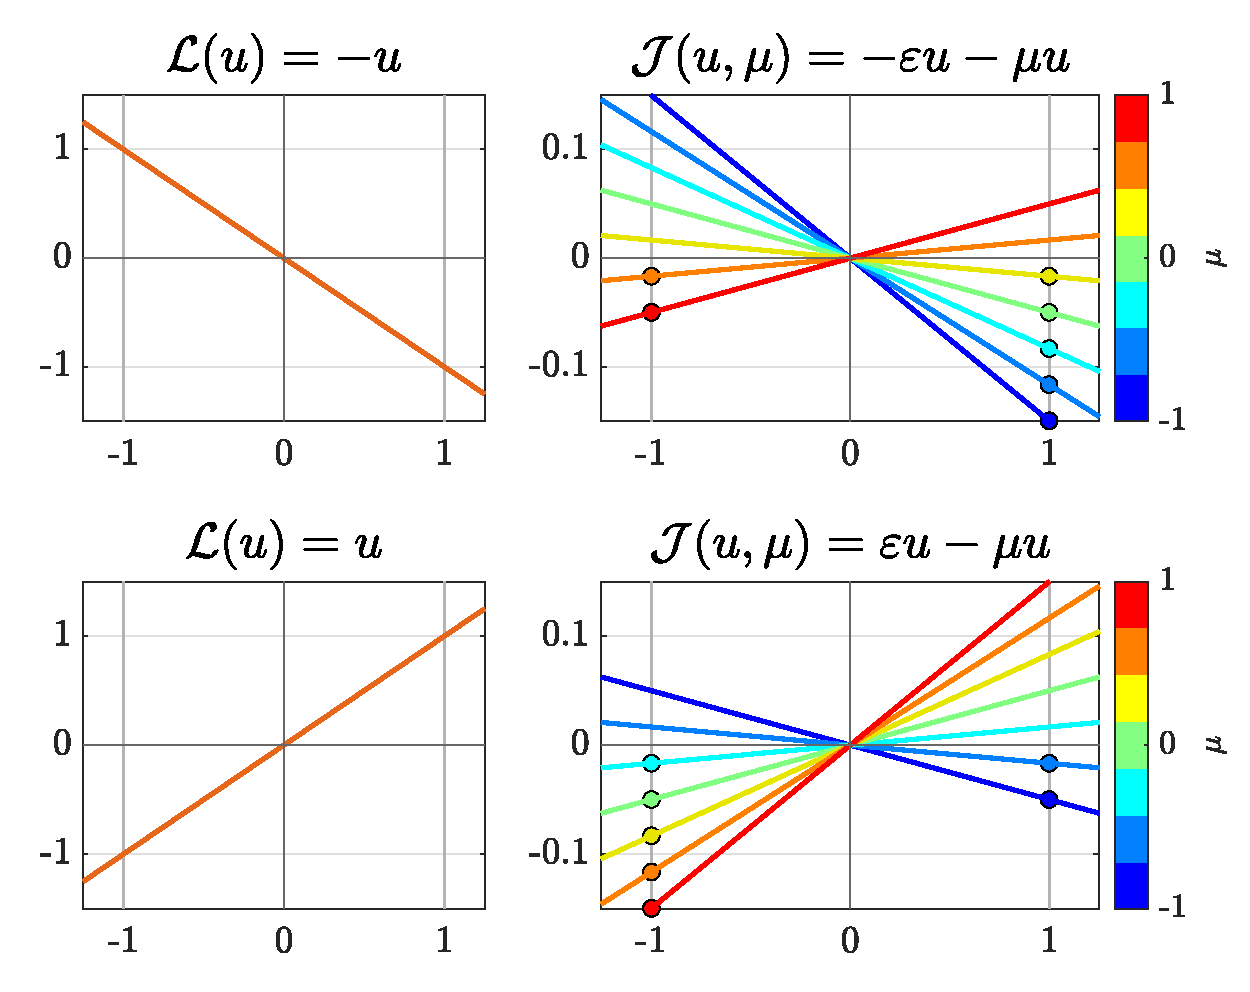
\includegraphics[scale=0.415]{img/fig03.eps}
    \caption{SHE bi-nivel via OCP (Bang-Bang Control)}
\end{figure}
\subsection{SHE multi-nivel via Piecewise linear penalization}

\begin{theorem}
    Dado un conjunto $\mathcal{U}$, we can choose the affine interpolation of a parabola $\mathcal{L}:[-1,1] \rightarrow \mathbb{R}$ as a penalization term. That is
    \begin{gather}\label{PLP}
        \mathcal{L}(u) = \begin{cases}
            \big[ (u_{k+1}+u_{k}) (u-u_k) + u_k^2 \big] & \text{if }  u \in [u_k,u_{k+1}[ \\
            1 & \text{if } u = u_{N_u} 
        \end{cases} \\
        \notag \forall k \in \{1,\dots,N_u-1\}
    \end{gather}
    De modo que el problema de \ref{pb:OCP2} con la penalización $\mathcal{L}(u)$ presentada antes tiene como solución un control digital del conjunto $\mathcal{U}$
\end{theorem}
\subsection{General conditions for  SHE multi-nivel}   

\begin{theorem}
    Assume that the finite set $\mathcal{U}$ defined in \eqref{eq:Udef} is composed by elements in ascending order. Let $\mathcal{Y} = \{y_\ell\}_{\ell=1}^L$ be another finite set, with the same cardinality as $\mathcal U$, such that the $L-1$ tuple
    \begin{gather}
        \frac{\Delta \mathcal{Y}}{\Delta \mathcal{U}} = \Bigg( \frac{y_\ell - y_{\ell+1}}{u_\ell - u_{\ell+1}} \Bigg)_{\ell=1}^{L-1}
    \end{gather}  is monotone. Let $\mathcal{L}:\mathbb{R} \rightarrow \mathbb{R}$ be a piece-wise continuous function:
    \begin{gather}
        \mathcal{L}(u) = \begin{cases}
            \mathcal{L}_k(u) & \text{if }  u \in [u_k,u_{k+1}[ \\
            1 & \text{if } u = u_{N_u} 
        \end{cases} \\
        \notag \forall k \in \{1,\dots,N_u-1\}
    \end{gather}    
    tal que $\{y_l = \mathcal{L}(u_l)\}_{l=1}^L$. Si las funciones $\mathcal{L}_k$ para todo $k \in  \{1,\dots,N_u-1\}$  son funciones concavas, entonces la penalización $\mathcal{L}$ en el problema \ref{pb:OCP2} da lugar a un control digital de $\mathcal{U}$.
\end{theorem}